
%%%%%%%%%%%%%%%%%%%%%%%%%%%%%%%%%%%%%%%%%%%%%%%%%%%%%%%%%%%%%%%%%%%%%%%%%%%%%

\section{Data structures}\label{app.datastructure}


The primary data structure in ENZO\ is the {\tt grid}.  
\gtt{It has yet to be determined how much of this
appendix will be in the Method Paper, and how much will be in the
User/Developer Guide.  Green type denotes text that will definitely be
in the User/Developer guide.} \red{Red denotes meta notes-- things to
write, fix, find.}

\subsection{Outline and List of Routines.}
\begin{enumerate}
 \item Creation and Destruction
   \begin{enumerate}
     \item Flow of Rebuild hierarchy: 
       \begin{enumerate}
	 \item delete hierarchy
	 \item build new hierarchy
	 \item scavange from old hierarchy
       \end{enumerate}
     \item Cell Flagging Methods
     \item Grid Fracturing Methods
   \end{enumerate}    
 \item Parallelism
  \begin{enumerate}
    \item Top Grid (block domain decomposition)
    \item Subgrids (memory balance, level by level)(Actually, I think
          its Parent Grid by Parent Grid.)
  \end{enumerate}
 \item Relation to other objects: 
   \begin{enumerate}
     \item Parents (No refinement jump requirements.  Talk about flux
        correction improvement to this effect here?)
     \item Siblings
     \item Children
     \end{enumerate}
 \item Traversing the hierarchy (this might be rolled into the
   previous bullet)
  \begin{enumerate}
    \item Level iterator 
    \item Hierarchy iterator
    \item Grid Array
    \item Chaining Mesh
  \end{enumerate}
  \item Particle treatement
   \begin{enumerate}
     \item Which grid gets the particles
     \item How particles are refined: criteria
     \item How particles are refined: how it fits in with the Grid refinement
   \end{enumerate}
  \item Ghost zones
    \begin{enumerate}
      \item how, when filled
    \end{enumerate}
  \item Timestepping
    \begin{enumerate}
      \item How timestep is determined
      \item Order of level operations: W cycle
    \end{enumerate}
\end{enumerate}
A list of routines to mention: \red{\zeus\ does this in a big table that
  references code name, what it does, and what equations it
  solves. Might be a useful idea to steal.}
\begin{description}
 \item[\tt{EvolveHierarchy}] Primary timestep control routine. 
 \item[\tt{EvolveLevel}] Primary evolution routine.
 \item[\tt{RebuildHierarchy}] Rebuilds the grid hierarchy
\end{description}

\subsection{Grid Intro}
The life of an \enzo\ simulation centers around the {\tt grid}
object and relationships between individual {\tt grid} instances.  
Grids are independant cartesian patches in space, which contain meta data about
that space (for instance its size, its position in the volume, 
size of the cells in that patch) as well as the data that belongs in
that space (fluid quntities like density and energy, as well as
particle quantites like position and velosity.)

Grids are treated, as individual instances of fluid
dynamics problems, with Dirichlet boundary conditions.  Boundary
conditions, stored in ghost zones, are determined by
one of 3 methods; from user defined exterior conditions like
outflow or reflecting, copied from active zones of 
neighbors, or interpolated from parents.  Grids are group in two
logical structures: a tree like hierarchy that relates parent grids to
children grids; and a level structure that relates grids of the same
refinement.  

\subsection{Creation and Destruction: \tt{RebuildHierarchy}}
Creation and destruction of grids happens in the routine
{\tt RebuildHierarchy}.  
At the end of every timestep, the Hierarchy is rebuilt.
Rebuilding starts at the coarsest level at the point in time (note
that coarser levels may be further ahead in their integration, due to
their larger timestep and the W-cycle)  Beginning with this coarsest level, each
grid on each level is examined for refinement.  Cells are first flagged
based on a variety of criterion, described in section
\ref{sec.flagging}.  The set of flagged cells, stored in the \grid\ memeber
array {\tt FlaggingField}, is then devided into grids as described
in section \ref{app.subgrid_creation}.  Data in these subgrids
is then created by interpolation from the parent using \red{what kind
  of interpolation?}  After this New Subgrid is filled with
interpolated data, the set of Old Subgrids is examined for overlapping
data.  All Old Cells that correspond to New Cells are coppied to the
New Grid.

\subsection{Cell Flagging Methods}\label{sec.flagging}
\enzo\ selects cells to refine based on the physics of the simulation.
Essentially any criterion that can be derived locally from the fluid
data and its derivatives can, in principal, be used to flag the cells
for refinement. Currently, \enzo\ has 8 methods of refinement.
installed, which we will discuss here.  Any or all of these methods may be employed in
any given \enzo\ simulation.  \gtt{Information on how to write your own
refinement criterion can be found Somewhere, to be written}
\begin{description}
  \item[Field Slope] \gtt{grid::FlagCellsToBeRefinedBySlope()} For each
  fluid quantity $u$, a cell $i$ is flagged if 
$$ \frac{u_{i+1}-u_{i-1}}{u_i} > slope $$
  where $slope$ \gtt{\tt MinimumSlopeForRefinement} is
  a  user-defined
  parameter. This is repeated for all
  3 directions. 
  \item[Baryon mass] \gtt{
  grid::FlagCellsToBeRefinedByMass()}  Cells
  are flagged if $$ \rho  V > m_{f} r^{\alpha L} $$ 
  where $V$ is the
  volume of the cell, $r$ is the refinement ratio, $L$ is the grid
  level, $m_{f}$ and ${\alpha}$ are user parameters. \gtt{MinimumMassForRefinement} and 
  \gtt{ MinimumMassForRefinementLevelExponent\[\]}
  \item[Baryon Overdensity] As the name suggests, refines if the
  density is greater than the mean density in the simulation.  In
  practice, this refinement method uses the same machenery as flagging
  by Baryon Mass, with the minimum
  mass for flagging, $m_f$ \gtt{ = MinimumMassForRefinement}, set to the
  input parameter \gtt{MinimumOverDensityForRefinement} times the
  mean density.  \gtt{This is calculted differently for each problem
  generator: consult the source for further documentation}
  \red{This could probably use a word on the effects of
  parameter choices.}
  \item[Shocks] \gtt{
  grid::FlagCellsToBeRefinedByShocks()} \red{This text should be
  updated to reflect Alexei's improvements} A cell $i$ is flagged if it is
  determined to be taking part in a shock.  This is determined if it
  has each of the following:
  \begin{enumerate}
    \item Large relative pressure jump: 
      $$\frac{|p_{i+1} - p_{i-1}| }{min( p_{i+1}, p_{i-1} ) }
      > \gtt{MinimumPressureJumpForRefinement} $$
     \item compression: $$ u_{i+1} < u_{i-1} $$
    \item More thermal energy than Kinetic: $$ \frac{
    \frac{p_i}{\gamma -1} }{ \frac{1}{2}\rho v^2 } > \gtt{
    MinimumEnergyRatioForRefinement } $$ \red{why?}
  \end{enumerate}  
  \item[Particle Mass] Using the Cloud In Cell interpolation method,
  described  \red{elsewhere?}, particle data is interpolated to the
  Eulerian grid cell centers.  A cell is flagged if the resulting mass field passes
  the ``RefineByMass'' test, described above.
  \item[Jeans Length] If a gravitationally collapsing simulation is
  under-resolved, artificial fragmentation can occur.  It was
  descoverd experimentally by \red{Truelove; get citation}
  that sufficient resolution was achieved if the Jeans Length is
  resolved by at least 4 cells.  This is determined if 
  $$ dx^2 >
  \frac{\alpha}{N_{cells} \gtt{= RefineByJeansLengthSafetyFactor}}\frac{T_{i,j,k}}{\rho_{i,j,k}} $$
  
  and $\alpha = \frac{\pi k_b }{G m_{proton} }*
  \frac{LengthUnits^2}{DensityUnits}$

  \red{dude, double check this.}
  \item[Cooling Time]  \red{Finish this.}

  \item[Shear] For highly turbulent flows, it may be useful to resolve
  shear layers.  This is done whenever
  $$\frac{\partial v_x}{\partial y}^2 + \frac{\partial v_x}{\partial z}^2 
  > \eta \gtt{= MinimumShearForRefinement}
  $$
  In practice, $$\frac{\partial v_x}{\partial y} = 
  u_{j+1}-u_{j-1}$$
  The same is done for $v_y$ and $v_z$
  
\end{description}

\subsection{Grid Fracturing}\label{app.subgrid_creation}
Once the cells in a given grid are flagged for refinement, they're
broken into a set of subgrids by an iterative process.  This process
first draws a minimally enclosing box around the set of flagging
cells, and generates a {\tt ProtoSubgrid}.  A {\tt ProtoSubgrid} is
essentially just the spatial extent and flagging field that will
define the spatial extent of the future \grid.  Each {\tt
  ProtoSubgrid} is then examined for efficiency (the ratio of flagged cells to
total), total size (for cache optimization) and minimum side
length (to avoid a flock of one zone grids).  {\tt ProtoSubgrid} that are too
large or not efficient enough are broken into smaller grids, by a
process to be described shortly, new minimally enclosing boxes are
drawn around each of the two remaining flagging fields, and new {\tt
  ProtoSubgrid}s are created.  This process is then repeated until
all {\tt ProtoSubgrid}s are both small enough and efficient enough.
It should be noted that \enzo\ does not glue grids back together-- the
Minimum Side Length is enforced by not examining the other two
conditions if the {\tt ProtoSubgrid} is too small.  

Maximum size, minimum side length,  and minimum efficiency are
controlled by the parameters {\tt MaximumSubgridSize}, {\tt MinimumSubgridEdge} and {\tt
  MinimumEfficiency}, respectivly. Typical maximum sizes are 10000 zones, minimum
side lengths are typically 5 zones, and minimum efficiencies are  0.2.
Choice of these parameters, especially maximum size, are
based on the architecture of the computer in question.  
Machines with larger cache sizes will benifit from larger values for
{\tt MaximumSubgridSize}, as communication and memory overhead from
ghost zones will be reduced; machines with smaller cache sizes benifit
from lower values, in that the computational time is reduced for a
grid that can fit entirely into cache.  

A {\tt ProtoSubgrid} that fails either the efficency or size
requirement is then broken into smaller {\tt ProtoSubgrid}s by a
method that tries to preserve physically continuous structures onto
individual grids.  The process examines the 1d Signature of the Flagging
field, which is the projection of the Flagging Field along two of the
coordinate axes.  First, each of the 3 signature fields is examined
for zeros.  Zeros in the signature field indicates disjoint
structures, so the {\tt ProtoSubgrid} is first cut into two smaller
ones along that line.  If no such cuts can be made, zero crossings of
the second derivative in the signature are then looked for.  Zero
crossings in the second derivative indicates edges of structures.  If
more than one exists, the ``strongest crossing'', that is the largest
jump, is selected for the cut.  If no such zero crossings can be
found, the {\tt ProtoSubgrid} is then cut evenly along the longest
axis.  See figure \ref{fig.signature} for a schematic of this process.

\begin{figure}
\begin{center}
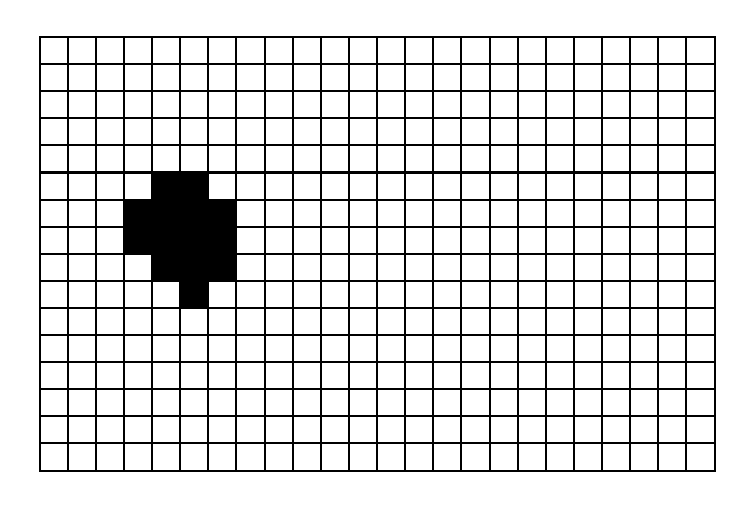
\includegraphics[width=0.4\textwidth]{figures/SignatureSchematic.eps}
\end{center}
\caption{
Schematic of Flagging Field and Signature.  Cuts will be made along
some line I'll draw.  The figure will be improved in the future.
}
\label{fig.signature}
\end{figure}





